\subsection{Parametric shape detection}

\subsubsection{Applications}
 
 Kong et alii. give the following application:
 
 Given a single image of an arbitrary road, that may not be well-pave, or have clearly delineated edges, or some a priori known color or texture distribution, is it possible for a computer to find this road?
 
\subsubsection{Hough for lines}

Intuitively, our algorithm will receive a set of edge points with the gradient magnitude and orientation on each of them and will output all straight lines in the image.

The first step towards the solution would be to cut the image in small pieces. Then, for each piece, estimate a line. Finally, group the lines, and keep the biggest groups.

The steps can be formalised in the following manner:

\begin{itemize}
\item Obtain binary edge points. To do so compute the gradient magnitude with the Sobel operator. Then, apply a threshold to get a binary edge map (with 0 and a max value for the gradient at each point).
\item Obtain candidate lines. Here we have to note that the cartesian formula for lines is not convenient, since vertical lines will have infinite slope. Instead we prefer the polar representation:

\begin{figure}[H]
\centering
\makebox[\textwidth][c]{
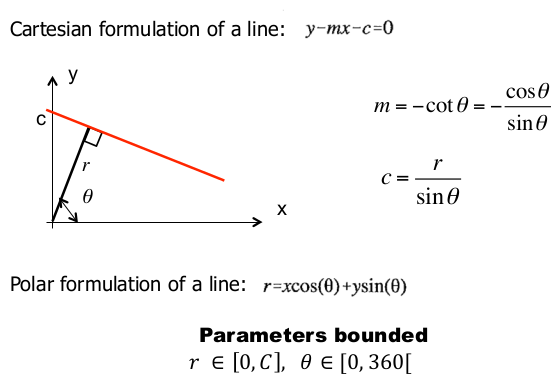
\includegraphics[scale=0.35]{./images/polar.png}
}
\end{figure}

After this, we discretize the parameter space and form an accumulator that will represent each of the resulting parameter discrete case. Then, for each edge point detected in the image space one increases the corresponding accumulator value.

\item Select the final Lines. The final question is how to precisely locate the intersection. We could use local maxima or non-max suppression:

\begin{itemize}
\item Local maxima: Pixel location whose value is bigger than any of its neighbouring values.
\item Non-Max Suppression: Keep local maxima that are large enough
\end{itemize}
\end{itemize}

\subsubsection{Other Hough (circle, ellipse, general)}

Given a parametric model of a curve:

\begin{itemize}
\item Map each edge point to the set of parameter values that define a curve passing through the point.
\item Find the maximum values in the resulting accumulator.
\end{itemize}

If we take a circle then the equation is $(x-x_0)^2 + (y-y_0)^2 = r^2$. Therefore, the accumulator has three parameters $(x_0,y_0,r)$. If we take an ellipse then the equation is $\frac{(x-x_0)^2}{a}+\frac{(y-y_0)^2}{b} = 1$. Therefore, the accumulator has four parameters $(x_0,y_0,a,b)$.

There is room for improvement. If we made votes depend on the direction of the edges of the shapes we could detect more general shapes. The tool for this is called R-table.

\subsubsection{Limitations}

Computational cost grows exponentially with the number of model parameters:

\begin{itemize}
\item Only works for objects whose shape can be defined by a small number of parameters.
\item Approach is robust but lacks flexibility.
\end{itemize}

\subsection{Blob detection}

Blob detection methods are aimed at detecting regions in a digital image that differ in properties, such as brightness or color, compared to surrounding regions. To achieve this a simple strategy is given as follows:

\begin{itemize}
\item Color segmentation: Create a binary image holding only the area of interest.
\item Connected Components: Connect the pixels to form blobs.
\end{itemize}

To perform color segmentation we can use several color spaces:

\begin{itemize}
\item RGB: The RGB color model is an additive color model in which red, green and blue light are added together in various ways to reproduce a broad array of colors. 
\item HSV: HSV stands for hue, saturation, and value, and is also often called HSB (B for brightness). In each cylinder, the angle around the central vertical axis corresponds to "hue", the distance from the axis corresponds to "saturation", and the distance along the axis corresponds to "lightness", "value" or "brightness". 
\end{itemize}

\begin{figure}[H]
\centering
\makebox[\textwidth][c]{
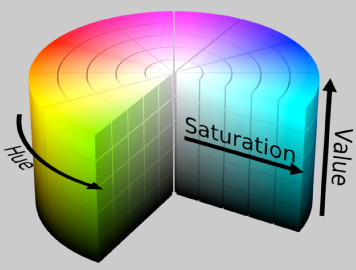
\includegraphics[scale=0.35]{./images/hsv.png}
}
\end{figure}

\subsubsection{Connected components algorithm}

Now we have our blobs, we need to group them to find the center. This relies on a two pass algorithm:

First pass: iterate through each element
 
If the element is not the background:

1.  Get the neighboring elements of the current element.\\
2.  If there are no neighbors, uniquely label the current element and
continue.\\
3.  Otherwise, find the neighbor with the smallest label and assign it.\\
4.  Store the equivalence between neighboring labels.\\

Second pass: iterate through each element

Assign smallest equivalent label.
 
\subsubsection{Limitations}

\begin{itemize}
\item Relies on a good first-hand thresholding.
\item Only works for objects with distinctive colors.
\item Errors in binary map generation (i.e. thresholding) can lead to multiple components for the same blob (and vice-versa).
\end{itemize}

\subsection{Other approaches}

Other approaches involve the laplacian of the gaussian, scale space blob detection, semantic segmentation, markov random fields and several tools from machine learning like classifiers and fully-convolutional neural networks.

\subsection{Summary}

Great progress made in shape and blob detection

\begin{itemize}
\item Learning-based methods currently most popular.
\item Semantic segmentation loses the notion of regions.
\item Pixels are treated independently.
\item Instance-level semantic segmentation.
\end{itemize}

\subsection{Exercises}

\begin{figure}[H]
\centering
\makebox[\textwidth][c]{
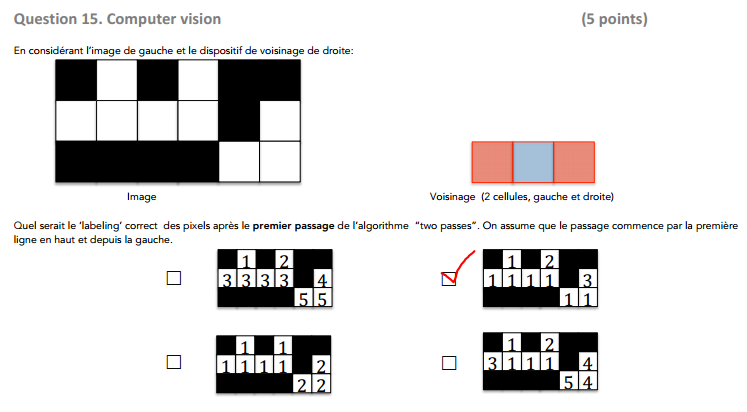
\includegraphics[scale=0.35]{./images/exercise51.png}
}
\end{figure}

\begin{figure}[H]
\centering
\makebox[\textwidth][c]{
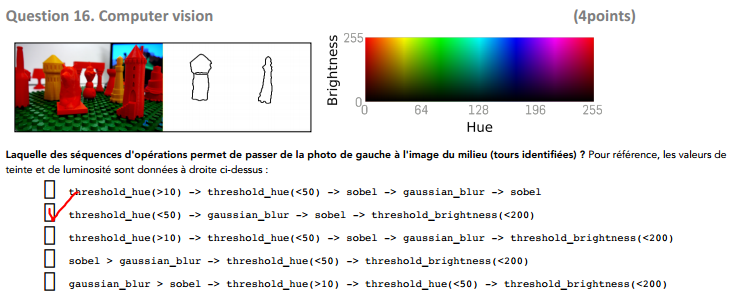
\includegraphics[scale=0.35]{./images/exercise52.png}
}
\end{figure}



































































